\documentclass[a4paper,12pt]{article}

\usepackage[T1]{fontenc}
\usepackage{graphicx} % for including graphics
\usepackage{longtable} % for tables that span multiple pages (if needed)
\usepackage[a4paper, top=2cm, bottom=2cm, left=2cm, right=1cm]{geometry}
\usepackage{pgfplots} % For plotting graphs
\usepackage[utf8]{inputenc}
\usepackage{listings}
\usepackage[serbian]{babel}

\definecolor{codegreen}{rgb}{0,0.6,0}
\definecolor{codegray}{rgb}{0.5,0.5,0.5}
\definecolor{codeblue}{rgb}{0.05,0.27,0.72}
\definecolor{backcolour}{rgb}{0.95,0.95,0.92}

\lstdefinestyle{mystyle}{
    backgroundcolor=\color{backcolour},   
    commentstyle=\color{codegreen},
    keywordstyle=\color{magenta},
    numberstyle=\footnotesize\color{codegray},
    stringstyle=\color{codeblue},
    basicstyle=\ttfamily\footnotesize,
    breakatwhitespace=false,         
    breaklines=true,                 
    captionpos=b,                    
    keepspaces=true,                 
    numbers=left,                    
    numbersep=5pt,                  
    showspaces=false,                
    showstringspaces=false,
    showtabs=false,                  
    tabsize=2
}



% Define your style
\lstdefinestyle{pisaniCstyle}{
    keywordstyle=\color{magenta}\ttfamily,
    basicstyle=\ttfamily\normalsize,
    keepspaces=true
}

% Adjust vertical space before and after code blocks
\lstset{
    aboveskip=10pt,    % Vertical space before code block
    belowskip=10pt     % Vertical space after code block
}

\title{OBARADA I ANALIZA MEDICINSKIH SLIKA \\ Smeinarski rad: Brojanje kvadrata}
\author{Ismar Osmanović / Lejla Zahirović}
\date{\today}

\begin{document}
\begin{center}
\thispagestyle{empty}
\large{UNIVERZITET U TUZLI \\ FAKULTET ELEKTROTEHNIKE}

\noindent\rule[7pt]{\linewidth}{0.4pt}


  
\includegraphics[width=0.7\linewidth]{fet_logo.png}
\vspace{3cm}\\
{\fontsize{34pt}{28pt}\selectfont SEMINARSKI RAD}\\
\large{OBARADA I ANALIZA MEDICINSKIH SLIKA}\\
\vspace{2cm}
\Huge{Tema:}\\
\Huge{Prepoznavanje kvadrata na slici}\\
\vspace{0.5cm}
\large{Ismar Osmanović / Lejla Zahirović}
\vfill

\noindent\rule[7pt]{\linewidth}{0.4pt}
\end{center}
\newpage
\tableofcontents
\newpage
\pagenumbering{arabic} 

\section{Ideja projekta}
\section{Realizacija projekta}
\lstinputlisting[language=matlab, style=mystyle, linerange={2}]{../brojanje_kvadrata_ciz.m}
\texttt{Imread} funkcija učitava sliku iz file-a koji je specificiran pomoću njegovog imena, utvrđujući format  na osnovu sadržaja istog. Ako je ime file-a file sa više slika, funkcija imread učitava prvu sliku u tom file-u.
Dakle, 'img/test1.jpg' je putanja do slike koja se učitava. img je varijabla u kojoj se čuva učitana slika. Nakon što je slika učitana, sadržaj slike (u formi matrice piksela) biće sačuvan u varijabli “img”. Ova funkcija je dio biblioteke koju koristi MatLab.

\lstinputlisting[language=matlab, style=mystyle, linerange={5}]{../brojanje_kvadrata_ciz.m}

Koristeći funkciju \texttt{rgb2hsv} slika se konvertuje iz RBG color prostora u HSV (Hue, Saturatiom, Value) color prostor. Dok RGB prostor koristi tri komponente (crvenu, zelenu i plavu) za reprezentaciju boja, HSV prostor koristi tri komponente:\\
\begin{itemize}
    \item Hue (boja slika kao crvena, plava),
    \item Saturation (intenzitet boje),
    \item Value(osvijetljenost boje).
\end{itemize}

Dakle, img je ulazna slika u RGB formatu, koja je pritome učitana pomoću \texttt {imread} funkcije, a “hsvImg” je promjenjljiva u kojoj će biti sačuvana slika u HSV formatu. \\

\indent Zašto je primjenjena ova konverzija, iz jednog color prostora u drugi, na ovom primjeru?\\

U opštem slučaju se u ovaj format koristi zbog svojih prednosti u obradi same slike. Naime, ovaj format pruža lakšu manipulaciju bojama. Naprimjer, H komponenta je nezavisna od svjetlosti i zasićenosti, pa je koristeći navedeni format lakše izolavati određene boje na slici, sto će kasnije biti primjenjeno, no isključivo koristeći RGB format. U implementaciji koda je upravo bio zadatak pronaći piksele crvene i zelene boje na datim slikama. Međutim, u prvobvitnom prostoru, taj zadatak bi bio znatno otežan jer bi bilo potrebno razmatrati sve tri komponente, a u ovom slučaju smo posmatrali samo H komponentu za filtriranje crvenih tonova, kao i zelenih. Preostale dvije mogu biti korištene za kontrolu jačine boje i osvjetljenosti. 

\lstinputlisting[language=matlab, style=mystyle, linerange={8-11}]{../brojanje_kvadrata_ciz.m}

Ove linije koda definišu pragove za filtriranje crvene boje u HSV color prostoru. Konkretno, koristi se Hue (H), Saturation (S) i Value (V) komponente za postavljanje opsega boje crvene(a kasnije i zelene), tako da se mogu prepoznati pikseli koji odgovaraju toj boji u slici.



\newpage


\begin{figure}
    \centering
    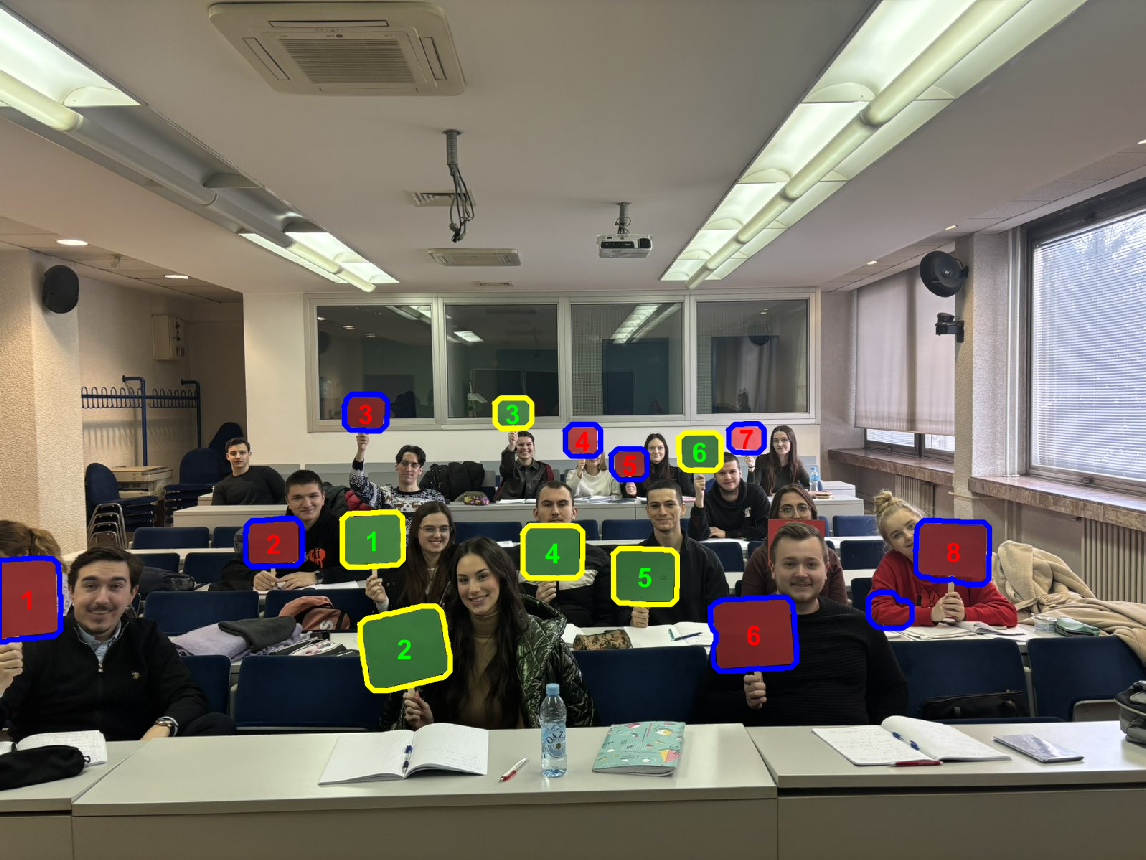
\includegraphics[width=\textwidth]{studenti.png}
    \caption{8 crvenih 6 zelenih}
    \label{fig:example}
\end{figure}

\end{document}
